\chapter{Technologien}
\label{sec:technologien}

Es gibt verschiedene Möglichkeiten Microservices zu implementieren. Möchte man diese erschließen, sollte man mindestens zwischen vier Ebenen in der Softwarehierarchie unterscheiden. Diese sind die genutzte Programmiersprache, die verwendeten Frameworks, der Aufbau der Architektur und die genutzte Protokolle in der Kommunikation mit dem Client. Da das Service-Orientated-Design, die Schichtenarchitektur und die Nutzung von \ac{REST} in Verbindung mit \ac{HTTP} bereits in der parallel zu dieser Arbeit geschriebenen Bachelorarbeit festgelegt wurden, wird in dieser Arbeit nur noch auf die Programmiersprache und die genutzten Frameworks eingegangen\autocite[Siehe][]{dnba}.  Zusätzlich zu der verwendeten Programmiersprache können auch unterschiedliche Bibliotheks- und Quellcodeverwaltungstools zur Unterstützung genutzt werden. Die bei der Implementierung des Prototypen der neuen Hochschul-\ac{App} verwendeten Programmiersprachen, Frameworks und Hilfstools werden im folgenden genauer betrachtet.

\section{Programmiersprache}
\label{sec:programmiersprache}
%http://pypl.github.io/PYPL.html
Bei der Wahl der Programmiersprache gilt es im Allgemeinen auf folgende Punkte zu achten:

\begin{itemize}
\item Allgemeine Beliebtheit
\item Nutzbarkeit der Sprache
\item Zuverlässigkeit der Sprache
\item Eignung für Anwendung
\item Programmiererfahrung in der Sprache
\end{itemize}

Da der Prototyp der Hochschul-\ac{App} in der Zukunft von Studierenden gepflegt und weiterentwickelt wird, werden für die Auswahl der Programmiersprache nur drei Möglichkeiten in Betracht gezogen, die in den Vorlesungen der Fakultät Informatik an der Hochschule auch gelehrt werden. Diese sind \ac{JS}, \ac{PHP} und Java.

\subsection*{Kandidaten}
Für ein besseres Verständnis der folgenden Bewertungen werden die drei Programmiersprachen kurz vorgestellt.

\subsubsection*{JavaScript} 

Der Autor Christian Wenz beschreibt die anfängliche Intention der Programmiersprache JavaScript wie folgt:

\begin{quote}
%seite 18 javascript zitiert
Mit JavaScript kann man die eher beschränkten Möglichkeiten von HTML erweitern. Es handelt sich bei JavaScript um eine clientseitige Programmiersprache. Das heißt, alles läuft im Browser ab, und man muss keine besonderen Server-Voraussetzungen erfüllen\autocite[][18]{javascript}.
\end{quote}

%seite 19 javascript ref
Ursprünglich wurde \ac{JS} 1995 von Netscape für deren Internet Browser in der Version 2.0 unter dem Namen LiveScript entwickelt. LiveScript war eine Programmiersprache, die dafür gedacht war, auf \ac{HTML}-Seiten Inhalte dynamisch zu manipulieren. Da die Syntax stark an die der Programmiersprache Java angelehnt war, wurde LiveScript später aus Marketinggründen zu JavaScript umbenannt, jedoch hat die Sprache bis auf die syntaktischen
Ähnlichkeiten keine weiteren Gemeinsamkeiten mit Java\footnote{Vgl. a.a.O S. 19}.
\\
\linebreak
Heute kann man mit \ac{JS} dank Frameworks wie \textit{Node.js} oder \textit{Angular} weitaus komplexere Anwendungen schaffen. So kann man nicht nur dynamisch \ac{HTML}-Inhalte manipulieren, sondern auch Contentmanagement betreiben oder ganze Serveranwendungen implementieren. 

\subsubsection*{Hypertext Preprocessor} 

%seite 31 php ref
Ursprünglich als Hobby-Projekt des Entwicklers Rasmus Lerdorf unter dem Namen \textit{Personal Homepage Tools} entstanden, entwickelte sich \ac{PHP} zu einer Programmiersprache mit der man einfach dynamische Webanwendungen erstellen kann. Anfangs bestand \ac{PHP} nur aus einer Sammlung von \textit{Perl}-Scripten die den Zugriff auf Webseiten protokollierten. Jedoch wurde der Funktionsumfang stetig erweitert, weshalb \ac{PHP} später aus Performanz gründen komplett in der Programmiersprache \textit{C} verfasst wurde\autocite[Vgl.][31\psqq]{php}.
\\
\linebreak
Heute zeichnet sich \ac{PHP} vor allem durch seine umfangreichen Funktionsbibliotheken und durch seine hervorragenden Anknüpfungsmöglichkeiten an Datenbanksysteme aus. \ac{PHP}-Scripte liegen ständig auf dem Webserver und werden nie mit dem statischen Content an den aufrufenden Client ausgeliefert. Sie werden bei einer Anfrage des Clients auf dem Server ausgeführt und liefern danach eine Antwort zurück. Somit eignen sich die \ac{PHP}-Scripte ebenfalls als eine Implementierungsmöglichkeit für Server.

\subsubsection*{Java} 

%seite 49f java ref
Java entstand in den 1970er Jahren als Wunsch des Softwareentwicklers Bill Joy, die Vorteile einiger bereits etablierten Programmiersprachen wie \textit{C} und \textit{Mesa} in einer neuen Sprache zu vereinen. Über einige Umwege entstand letztendlich die Programmiersprache \textit{Oak} die schlussendlich 1994 den Namen Java bekam\autocite[Vgl.][49\psq]{java}.

%seite 51 java zit
\begin{quote}
Java ist eine objektorientierte Programmiersprache, die sich durch einige zentrale Eigenschaften auszeichnet. Diese machen sie universell einsetzbar und für die Industrie als robuste Programmiersprache interessant. Da Java objektorientiertes Programmieren ermöglicht, können Entwickler damit relativ einfach moderne und wiederverwertbare Softwarekomponenten entwickeln\footnote{a.a.O S. 51}.
\end{quote}

In den folgenden Kapitel werden die Programmiersprachen untereinander verglichen und auf ihre Verwendbarkeit für den Prototypen der neuen Hochschul-\ac{App} analysiert.

\subsection*{Allgemeine Beliebtheit} 

Bei der Wahl der Programmiersprache sollte unter anderem auch auf die allgemeine Beliebtheit der Sprache geachtet werden, da diese die Weiterentwicklung der Anwendung maßgeblich beeinflussen kann. Sollte eine Sprache verwendet werden, die im Trend immer schlechter bewertet wird und kaum noch genutzt wird, so könnten die Studierenden in der Zukunft das Interesse an der Weiterentwicklung der Anwendung verlieren.\\
\linebreak
Hierbei sticht vor allem die Sprache Java deutlich heraus. Laut dem \ac{PYPL} liegt Java im Gesamtvergleich aller Programmiersprachen auf Platz 2 mit etwa 19\% des Anteils der Suchen von Programmiersprachen auf der Suchplattform \textit{Google}. Doch auch \ac{JS} (Platz 3, ~8\%) und \ac{PHP} (Platz 5, ~6\%) können sich laut \ac{PYPL} durchaus als beliebt bezeichnen\autocite[][]{pypl}. Anhand der Werte ist zu erkennen, dass alle drei Sprachen grundsätzlich geeignet sind, Java hier prozentual jedoch klar besser abschneidet als \ac{JS} und \ac{PHP}.\\
\linebreak
Anzumerken ist hierbei, dass \ac{PYPL} lediglich die Suchanfragen der Stichwörter zu den Programmiersprachen auf der Suchmaschine \textit{Google} untersucht und daraus die Beliebtheit der Sprachen ableitet. \ac{PYPL} nimmt dabei an, dass eine Programmiersprache umso beliebter ist, wenn sie oft in Verbindung mit Suchanfragen im Internet zu finden ist\footnote{ebd.}. Als Messwert für die Beliebtheit einer Sprache für die Auswahl der Programmiersprache in dieser Arbeit soll dieser Wert aber genügen.

\subsection*{Nutzbarkeit der Sprache} 

Ähnlich zur Beliebtheit einer Programmiersprache bietet die Nutzbarkeit der Sprachen einen weiteren wichtigen Punkt zur Entscheidungsfindung. Unter Nutzbarkeit ist in diesem Kontext der Schreibfluss, die Einfachheit des Syntax und die vorhandene Dokumentation einer Sprache zu verstehen. Des weiteren sollten auch die nötigen Rahmenbedingungen und Vorbereitungen für die Nutzung der Sprache sowie die benötigten \acp{LOC} für das Erfüllen einer bestimmten Aufgabe betrachtet werden. Auch die Lizenzierung der Sprachen spielt bei der Nutzung in einer Hochschulumgebung eine wichtige Rolle.\\
\linebreak
Der Schreibfluss bei den Sprachen Java, \ac{JS} und \ac{PHP} unterscheidet sich nur minimal. \ac{JS} lehnt seine Syntax sogar an der von Java an. Auch \ac{PHP} orientiert sich an einer ähnlichen Syntax, störend wirkt hier lediglich das \textit{\$}-Zeichen vor den Variablen, was je nach Tastatur Layout schwieriger zu tippen ist. Den größten Schreibfluss hat man wohl bei \ac{JS}, da dort Typisierung und störende Sonderzeichen komplett wegfallen. Jedoch ist das eine rein subjektive Auffassung und kann von anderen durchaus anders eingeschätzt werden. Die Dokumentation ist bei allen Sprachen hervorragend, wobei sich hier auch Java durch seine starke Community auszeichnet.\\
\linebreak
Bei der Nutzung der Sprachen und den nötigen Rahmenbedingungen stellt sich die Sprache \ac{JS} als hervorragend dar, da für die Nutzung dieser Sprache lediglich ein Web-Browser von Nöten ist. Für Java wird hingegen eine Laufzeit- beziehungsweise eine Entwicklungsumgebung benötigt, bei \ac{PHP} ein Server mit den benötigten Installationspaketen. Das schnelle Lösen von Aufgaben mit möglichst wenigen \acp{LOC} ist die Stärke von \ac{PHP}, da die Sprache eine breite Auswahl an Bibliotheken und Funktionen bereits im Sprachumfang enthalten hat.\\
\linebreak
Bei der Lizenzierung gibt es für die Sprachen \ac{PHP} und \ac{JS} keine Probleme, für Java kann die Open-Source Implementierung OpenJDK statt der originalen Version, die unter Oracle lizenziert ist, verwendet werden. Somit fällt bei der Nutzbarkeit der Sprachen kein Kandidat aus der Auswahl heraus. Anzumerken ist, dass vor allem \ac{JS} leicht zu verwenden ist, jedoch Java hier die Grundlage für de Syntax bietet. Auch die statische Typisierung der Sprache Java macht es Entwicklern leichter, fehlerfreie Software zu schreiben.

\subsection*{Zuverlässigkeit der Sprache} 

Bei der Zuverlässigkeit einer Sprache geht es vor allem um die Fehleranfälligkeit der Software, die in dieser Sprache geschrieben wurde. Hierbei ist vorweg zu sagen, dass die meisten unerwarteten Fehler durch eine fehlende Typisierung oder durch schwer lesbare Code-Abschnitte verursacht werden. Da bei der Programmiersprache Java die statische Typisierung gegeben ist und die Syntax eindeutig ist, liegt die Sprache in dieser Kategorie klar vorne. \ac{JS} und \ac{PHP} haben hier das Problem, dass in der ursprünglichen Fassung der Sprachen eine Typisierung nicht vorgesehen war und erst später durch Zusätze versucht wurde, diese einzufügen oder zumindest die Fehleranfälligkeit dieser Sprachen durch nicht-typisierte Variablen zu minimieren. Zudem bieten beide Sprachen mehrere Möglichkeiten einfache Probleme durch unterschiedlichen Syntax zu lösen, was bei der Programmierung eventuell zu Problemen führen kann. Auch die Einschätzungen dieses Absatzes sind jedoch subjektiv und müssen nicht von jedermann akzeptiert werden.

\subsection*{Eignung für Anwendung} 

Für die Eignung der Anwendung qualifiziert sich klar die Programmiersprache Java. Es ist zwar durchaus möglich, in \ac{JS} und \ac{PHP} Web-Server zu schreiben, der Ursprung beider Sprachen liegt aber in der Manipulation von \ac{HTML}-Content. Java hingegen bietet durch Java \textit{EE} und andere Spracherweiterungen nativ die Grundlagen, Web-Server zu implementieren. Durch die Laufzeitumgebung von Java ist es auch einfach, auf Servern mit hoher Rechenkraft aufwändige Anfragen zu bearbeiten. Des weiteren bieten Drittanbieter einige Frameworks für Java, die genau auf die Bedürfnisse von Web-Anwendungen ausgelegt sind.

\subsection*{Programmiererfahrung in der Sprache} 

Als letzter Punkt soll die allgemeine Programmiererfahrung der Studierenden der Hochschule Hof betrachtet werden, denn diese ist ausschlaggebend dafür, welche Sprachen in Zukunft für die Pflege und Weiterentwicklung der Anwendung in Frage kommen. Auch hier stellt sich Java in den Vordergrund, da Java in der Fakultät Informatik als Einstieg in die Programmierung genutzt wird. Weiterführende Vorlesungen bauen dann oft auf den in der Programmiersprache Java gelernten Kenntnissen auf. Sowohl \ac{JS} und \ac{PHP} werden je nach lehrenden Dozenten zwar auch behandelt, jedoch nur selten als Hauptsprache einer Vorlesung, weshalb die Kenntnisse hier innerhalb der Studierenden stark schwankt.

\subsection*{Fazit}

Trotz der Attraktivität der Sprachen \ac{JS} und \ac{PHP} im Bereich der Web-Program\-mierung und der Nutzung im Allgemeinen fällt die Wahl der Programmiersprache für den Prototypen der neuen Hochschul-\ac{App} klar auf Java. Die Kenntnisse der Studierenden der Hochschule sowie die hohe Zuverlässigkeit der Sprache und die Eignung für den Anwendungsfall des Web-Servers überwiegen hier klar.

\section{Microservice Framework}
\label{sec:framework}

Im Bereich der Server-seitigen Programmierung in Java haben sich im Laufe der letzten Jahre einige Frameworks zur Unterstützung typischer Webanwendungen etabliert. Dabei fokussieren sich diese Frameworks im allgemeinen auf verschiedene Use-Cases, zu denen zum Beispiel leichtgewichtige Anwendungen, große Serverimplementierungen oder auch große Anwendungen, die aber wenig Daten im Hintergrund halten, gehören. Um etwas genauer auf die Wahl des Frameworks einzugehen, werden kurz einige davon aufgelistet und deren Use-Cases dargestellt.\\

\begin{itemize}
\item \textbf{Spring Boot}\\
\textit{Spring Boot} ist ein Framework, das darauf ausgerichtet ist, komplexe Strukturen in einer Web Applikation einfach erstellen zu können und die Konfigurierung der Ressourcen so einfach wie möglich zu halten. Wegen der breiten Einbindung anderer Frameworks für Dinge wie Datenbankanbindung, Discovery Services und andere Hilfsmittel bietet \textit{Spring Boot} eine gute Grundlage für die schnelle Entwicklung einer großen Anwendung. \textit{Spring Boot} ist vor allem bekannt durch seine Einsatzmöglichkeiten im Microservice Bereich in Verbindung mit \ac{REST}-\acp{API}\autocite[][]{spring_boot}.

\item \textbf{Struts}\\
\textit{Struts} ist ein open-source Framework, welches für moderne Web Anwendungen entwickelt wurde. Durch eine Plug-In Architektur soll \textit{Struts} die Einbindung anderer Bibliotheken, beziehungsweise die Entwicklung neuer Schnittstelle,n deutlich vereinfachen. Struts ist nicht zwingend für Microservices ausgelegt und kann weit mehr als nur \ac{REST}-Anwendungen unterstützen\autocite[][]{struts}.

\item \textbf{Kumuluz \ac{EE}}\\
\textit{Kumuluz \ac{EE}} ist ein open-source Microservice Framework. Im Gegensatz zu \textit{Spring Boot} legt \textit{Kumuluz \ac{EE}} seinen Fokus auf auf die Entwicklung leichtgewichtiger Web Anwendungen, wobei auch hier Schnittstellen für leichtgewichtige Erweiterungen geboten werden\autocite[][]{kumuluz}.

\item \textbf{\ac{JAX-RS}/ Jersey}\\
\textit{Jersey} ist eine Implementierung von \textit{\ac{JAX-RS}}, eine Bibliothek, welche darauf abzielt, einen Standard für die Entwicklung von Java \ac{REST} Services mit Java \ac{EE} zu bereitzustellen. Da dieser Standard so viele Funktionen wie möglich unterstützen soll, ist er sehr mächtig, im gleichen Zug allerdings auch deutlich aufwändiger in der Nutzung. Des weiteren wurde \textit{\ac{JAX-RS}} auch dafür entwickelt, sowohl den Server als auch die benötigten Clients in Java zu implementieren\autocites[][]{jaxrs}[][]{jersey}.

\end{itemize}

\subsection*{Kriterien bei der Framework Wahl}
\label{sec:kriterien_framework}

Die oben genannten Frameworks sind nur eine Auswahl der bekanntesten und der meist genutzten Frameworks für Web Anwendungen. Da hier eine große Auswahl für die Entwickler zur Verfügung steht, bedarf es eine Sammlung von Funktionen, die das endgültig gewählte Framework auch beherrschen muss. Zudem gibt es auch noch einige Kriterien, die die Frameworks erfüllen sollten. Diese Funktionen und Kriterien werden hier kurz aufgelistet und erläutert.

\begin{itemize}

\item \textbf{Startzeiten}\\
Jeder Webserver muss an mehreren Punkten in seinem Lebenszyklus auch gestoppt und gestartet werden. Ist ein Server gestoppt, so kann er seine Funktionen nicht erfüllen. Diesen Zeitraum, in der ein Server keine Anfragen bearbeiten kann, nennt man \textit{Downtime}. Im Falle des Prototypen der neuen Hochschul-\ac{App} sollte sich diese \textit{Downtime} möglichst auf die Nacht beschränken. Sollte der Server dennoch aus unerwarteten Gründen in den Hauptnutzungszeiten gestoppt werden, so ist es durchaus wichtig, wie schnell er neu gestartet werden kann. Da sich die voraussichtliche Nutzung der neuen Hoch\-schul-\ac{App} auf wenige Tausend Studierende beschränken wird ist dieses Kriterium lediglich für die Weiterentwicklung relevant, da kurze Ausfallzeiten von ein paar Minuten durchaus vertretbar sind.

\item \textbf{Erste Anfrage}\\
Jeder der oben genannten Frameworks unterstützt Caching Mechanismen, die es erlauben, Daten zwischenzuspeichern, sobald sie einmal von einem Client abgefragt wurden. Das ist vor allem bei Daten sinnvoll, die sich selten ändern, da so nicht die komplette Schichtenarchitektur bis zur Datenbank des Servers durchlaufen werden muss, um die benötigten Daten abzufragen. Jedoch werden Daten in der Regel erst im Cache abgelegt, wenn sie das erste mal abgefragt wurden. So ist die Bearbeitungszeit so einer Anfrage durchaus von Relevanz. Im Falle der Hochschul-\ac{App} ist dieses Kriterium durchaus relevant, aber nicht ausschlaggebend für die Wahl des Frameworks. Die meisten Daten können gecached werden, jedoch hält sich die allgemeine Komplexität der Datenabfrage in Grenzen, was die Bearbeitungszeit von Anfragen gering hält.

\item \textbf{Antwortzeiten bei kleinen Datenmengen}\\
Wie im Punkt \textit{Erste Anfrage} bereits erwähnt wurde, liegt bei Web Server Implementierungen der Fokus auf Antwortzeiten. Dabei muss man oft die Art der Anfrage unterscheiden. Neben der ersten Anfrage einer Ressource und der Anfrage einer Ressource aus dem Cache muss man noch zwischen den angefragten Datenmengen unterscheiden. Dabei ist es irrelevant, ob die Daten gecached sind oder nicht. Kleinere Datenmengen sollten mit minimalem Zeitversatz beantwortet werden. Das ist vor allem auch bei der Hochschul-\ac{App} wichtig, denn dort werden in der Regel nur kleinere Datenmengen abgefragt, die dann aber auch möglichst schnell auf den Endgeräten der Studierenden angezeigt werden sollen

\item \textbf{Antwortzeiten bei großen Datenmengen}\\
Im Gegensatz zu den Antwortzeiten bei kleineren Datenmengen ist diese bei größeren Datenmengen im Falle der neuen Hochschul-\ac{App} weniger relevant. Es kann zwar durchaus vorkommen, dass große Datensätze angefragt werden, das sollte aber nur bei der Einrichtung der Nutzerpräferenzen und der personalisierten Daten vorkommen. Da das pro Nutzer in der Regel nur einmal passiert, sind die Antwortzeiten bei Anfragen mit großen Datenmengen weniger relevant.

\item \textbf{Verhalten bei Hochlast}\\
Jede Web Anwendung hat sehr wahrscheinlich einen Zeitraum, in der überdurchschnittlich viele Nutzer auf sie zugreifen. In dieser Zeit ist es kritisch, die Anfragen trotz der hohen Last schnell beantworten zu können, da man sonst die Nutzer abschreckt und sich zusätzlich verwundbar für \ac{DoS} und \ac{DDoS} Angriffe macht. Bei der neuen Hochschul-\ac{App} ist davon auszugehen, dass solche Stoßzeiten früh am Tag vor der ersten planmäßigen Vorlesung und durchaus auch später am Tag vor der Mittagspause entstehen können. Trotz der geringen Gesamtnutzerzahl sollte nun darauf geachtet werden, das die Webserver der Anwendung auch unter Last nur geringe Ressourcen verbrauchen, da noch nicht klar ist, wie mächtig die darunterliegende Hardware ist.

\item \textbf{Einfachheit der Entwicklung}\\
Der wohl ausschlaggebende Punkt bei der Wahl des passenden Frameworks für den Prototypen der neuen Hochschul-\ac{App} ist die Einfachheit der Nutzung dieses Frameworks. Möchte man eine Anwendung schaffen, die im Umfeld von Studierenden, die ihr sich ihr professionelles Wissen erst aneignen, weiterentwickelt werden soll, so sollte man sich auf einfache und doch mächtige Techniken beschränken.

\end{itemize}

\subsection*{Entscheidungsfindung}

Grundsätzlich erfüllen alle der oben genannten Frameworks die Kriterien aus Kapitel \ref{sec:kriterien_framework}, besonders bei der erwartet geringen Nutzung der Anwendung aufgrund der Größe der Hochschule Hof. Dennoch erweist sich das \textit{Spring Boot} Framework besonders für die Implementierung der neuen Hochschul-\ac{App}. Die Gründe hierfür werden im folgenden kurz erläutert.

\subsubsection*{Hervorragende Dokumentation}
\textit{Spring Boot} verfügt über eine hervorragende Dokumentation. Dies zeigt sich hauptsächlich durch zwei Gründe. Der erste ist die sehr simple und umfangreiche Dokumentation, die \textit{Spring Boot} von sich aus zur Verfügung stellt. Der zweite ist die große Community, die durch die Popularität des Frameworks stetig am wachsen ist. Durch diese Community sind einige Foren entstanden, in denen viele häufig auftretende Probleme bei der Entwicklung diskutiert werden.

\subsubsection*{Kompatibilität}
\textit{Spring Boot} liefert von Haus aus eine große Liste von unterstützten Frameworks mit sich. Dazu gehören unter anderem Hibernate (eine \ac{JPA} Implementierung), Zuul (\ac{API}-Gateway) und JUnit5 (Testframework). Des weiteren ist die Einbindung anderer Frameworks durch die Nutzung von Maven \footnote{Siehe \ref{sec:build_tool}} sehr einfach gestaltet.

\subsubsection*{Abstrahierung}
Web Anwendungen sind oft voller komplexer Konzepte, speziell in Verbindung mit Java \ac{EE}. Hierbei wird oft auf komplizierte Annotations, Dependency Injection und Beans gesetzt. Die Nutzung solcher Konzepte ist grundsätzlich unterschiedlich zu der normalen Verwendung der Programmiersprache Java. Des weiteren werden diese Konzepte nur geringfügig in den Vorlesung der Fakultät Informatik der Hochschule Hof gelehrt. \textit{Spring Boot} vereinfacht die Nutzung dieser Konzepte durch die Einführung der Auto-Konfiguration und vereinfachten Annotations. Dies macht Spring sehr mächtig und dennoch leicht nutzbar für Entwickler mit beschränkter Programmiererfahrung.

\subsubsection*{Einfache Nutzung}
\textit{Spring Boot} bietet ein Web-Service an, der es Nutzern erlaubt, Projekte, die mit \textit{Spring Boot} implementiert werden sollen, über eine Webseite zu erstellen und sie dann vorkonfiguriert herunterzuladen. Dieser Service heißt \textit{Spring Initializr [sic!]}\autocite[Siehe][]{initializr}. Nach dem Herunterladen des voreingestellten Projektes können Feineinstellungen dann über sogenannte \textit{Property Files} vorgenommen werden.\\
\linebreak
Aufgrund der oben genannten Vorteile des \textit{Spring} Frameworks wird dieses zur Implementierung des Prototypen der neuen Hochschul-\ac{App} genutzt. Anzumerken ist hier auch, dass die Entwickler des Prototypen bereits Erfahrung bei der Nutzung von \textit{Spring Boot} haben, was auch in die Entscheidungsfindung eingeflossen ist. Des weiteren ist festzuhalten, dass die Anwendung prinzipiell mit allen oben genannten Frameworks gut implementiert werden kann, dennoch muss das Niveau der Programmierung von Studierenden mit in Betracht gezogen werden, weshalb \textit{Spring Boot} durch seine Einfachheit und der trotzdem enthaltenen Mächtigkeit die beste Wahl ist. Genaueres zur Konfiguration und Details zum Framework \textit{Spring Boot} wird in Kapitel \ref{sec:konfig} beschrieben.

\section{Build Management Tool}
\label{sec:build_tool}

Zur einfachen Einbindung von neuen Bibliotheken und zur Konfiguration des Build Prozesses benötigt der Prototyp der neuen Hochschul-\ac{App} ein sogenanntes Build Management Tool. Die bekanntesten Vertreter dieser Tools sind aktuell Gradle, Maven und Ant. Diese Vertreter sollen nun kurz betrachtet werden, worauf dann die Entscheidung für eines der drei Tools begründet wird.

\begin{itemize}
\item \subsection*{Ant}
%Seite 37 xtreme 
\textit{Ant} ist ein Build Management Tool das von der Apache Software Foundation entwickelt wurde. Es erlaubt seinen Nutzern, den Build Prozess einer Anwendung zu automatisieren. Zudem ist anzumerken, dass \textit{Ant} speziell für Java Anwendungen entwickelt wurde. Der große Vorteil von \textit{Ant} ist seine Erweiterbarkeit, denn man kann mit selbst entwickelten Java Tasks die Automation immer weiter verfeinern\autocite[Vgl.][37]{xtreme}.

\item \subsection*{Gradle}
Im Gegensatz zu \textit{Ant} ist \textit{Gradle} ein Build Management Tool, welches dafür entwickelt wurde, jede Art von Software zu unterstützen. \textit{Gradle} ist ein open-source Projekt, das in der \ac{JVM} Umgebung läuft. Das soll den Kennern der Sprache Java ermöglichen, Erweiterungen für \textit{Gradle} zu entwickeln.\autocite[][]{gradle}

\item \subsection*{Maven}
%Seite 457 xtreme 
\textit{Maven} ist aus dem Wunsch heraus geboren, einfach neue Funktionalitäten in einen Build-Prozess während einer Entwicklung einer Anwendung hinzuzufügen. Solche Funktionalitäten können beispielsweise Unit-Tests oder das Erfassen von Codemetriken sein. Die Anfänge von \textit{Maven} bauen auf \textit{Ant} auf. Jedoch nutzt \textit{Maven} mittlerweile \textit{Jelly} als primären Scripting-Engine. Die Stärke von \textit{Maven} ist es vor allem, mächtige \textit{Ant} Skripte mit in den Build Prozess aufzunehmen\autocite[Vgl.][457]{xtreme}. Des weiteren bietet Apache ein mächtiges Verzeichnis an, das es ermöglicht, Bibliotheken in verschiedensten Versionen per \textit{Maven Dependency} automatisiert in das Projekt mit einzubinden.

\end{itemize}

\subsection*{Entscheidungsfindung}

Für den Prototypen der neuen Hochschul-\ac{App} wird das Build Management Tool \textit{Maven} genutzt. Ein Vorteil dessen ist, das \textit{Spring Boot} in seinem \textit{Spring Initializr} das Erstellen von sowohl \textit{Maven}- als auch \textit{Gradle}-Projekten unterstützt. \textit{Maven} bietet sich aus diesen zwei Möglichkeiten deshalb an, da es unter anderem sehr leicht und intuitiv zu nutzen ist. Außerdem kann man mit \textit{Maven} sehr einfach \textit{Ant} Skripte einbinden.

\section{Versionsverwaltung Tool}
\label{sec:git}

Jedes Projekt, ob nun kollaborativ erstellt oder in Eigenarbeit geschaffen, benötigt ein Versionsverwaltung-Tool, idealerweise mit der Möglichkeit den Source Code auf externen Servern zu speichern, um Verluste durch einen Ausfall des Entwickler-Computers zu vermeiden. In der heutigen Zeit kommen dabei in der Regel nur noch zwei Kandidaten in Betracht, \textit{git} und \textit{Mercurial}. Für dieses Projekt gilt \textit{git} jedoch als einzig sinnvolle Option. Das liegt vor allem daran, dass die Hochschule einen eigenen GitLab Server besitzt, welcher es ermöglicht, Projekte, die über \textit{git} verwaltet werden, zu synchronisieren und auf dem Hochschul Server zu speichern. Des weiteren ist \textit{git} das weltweit wohl verbreitetste Versionsverwaltung-Tool. Auch der Lehrinhalt der Vorlesungen der meisten Dozenten der Hochschule Hof beinhaltet lediglich das Tool \textit{git}.

\section{API Gateway}

Wie in der parallel verfassten Bachelorarbeit bereits ausführlich erläutert wurde, besteht die Architektur der neuen Hochschul-\ac{App} aus mehreren Microservices, die die implementierten Funktionalitäten jeweils kapseln\autocite[][]{dnba}. Um dennoch eine einheitliche Anwendung zu schaffen, die nach außen nur eine Schnittstelle hat, wird ein sogenanntes \ac{API}-Gateway verwendet, das als Fassade zu den einzelnen Services dienen soll. Diese Microservices sind in folgende Funktionalitäten gekapselt:

\begin{itemize}
\item Stundenplan
\item Planänderung
\item Speiseplan
\item Benachrichtigungen
\item Sicherheit
\item Anwenderverwaltung
\item Sprachzentrum
\item Termine
\end{itemize}

Jedoch ist enthält der Umfang dieser Arbeit lediglich die Stundenplaninformationen, Stundenplanänderungen Mensadaten und den Benachrichtigungsservice. Alle anderen Services werden in einer anderen Abschlussarbeit separat entwickelt. Um die Anbindung der restlichen Services zu ermöglichen, ohne dass sich die Schnittstelle nach außen ändert, dient ebenfalls das \ac{API}-Gateway. Das Gateway ermöglicht es ebenfalls, zusätzlich zur Fassaden-Funktion, ein Load-Balancing der einzelnen Services zu konfigurieren, wenn diese redundant auf mehreren physischen Instanzen laufen. Die Auswirkung, die bei der redundanten Haltung der Service-Instanzen in Kombination mit der Microservice-Architektur anfallen würden, sind in der folgenden Abbildung bildlich dargestellt.

\begin{figure}[H]
\centering
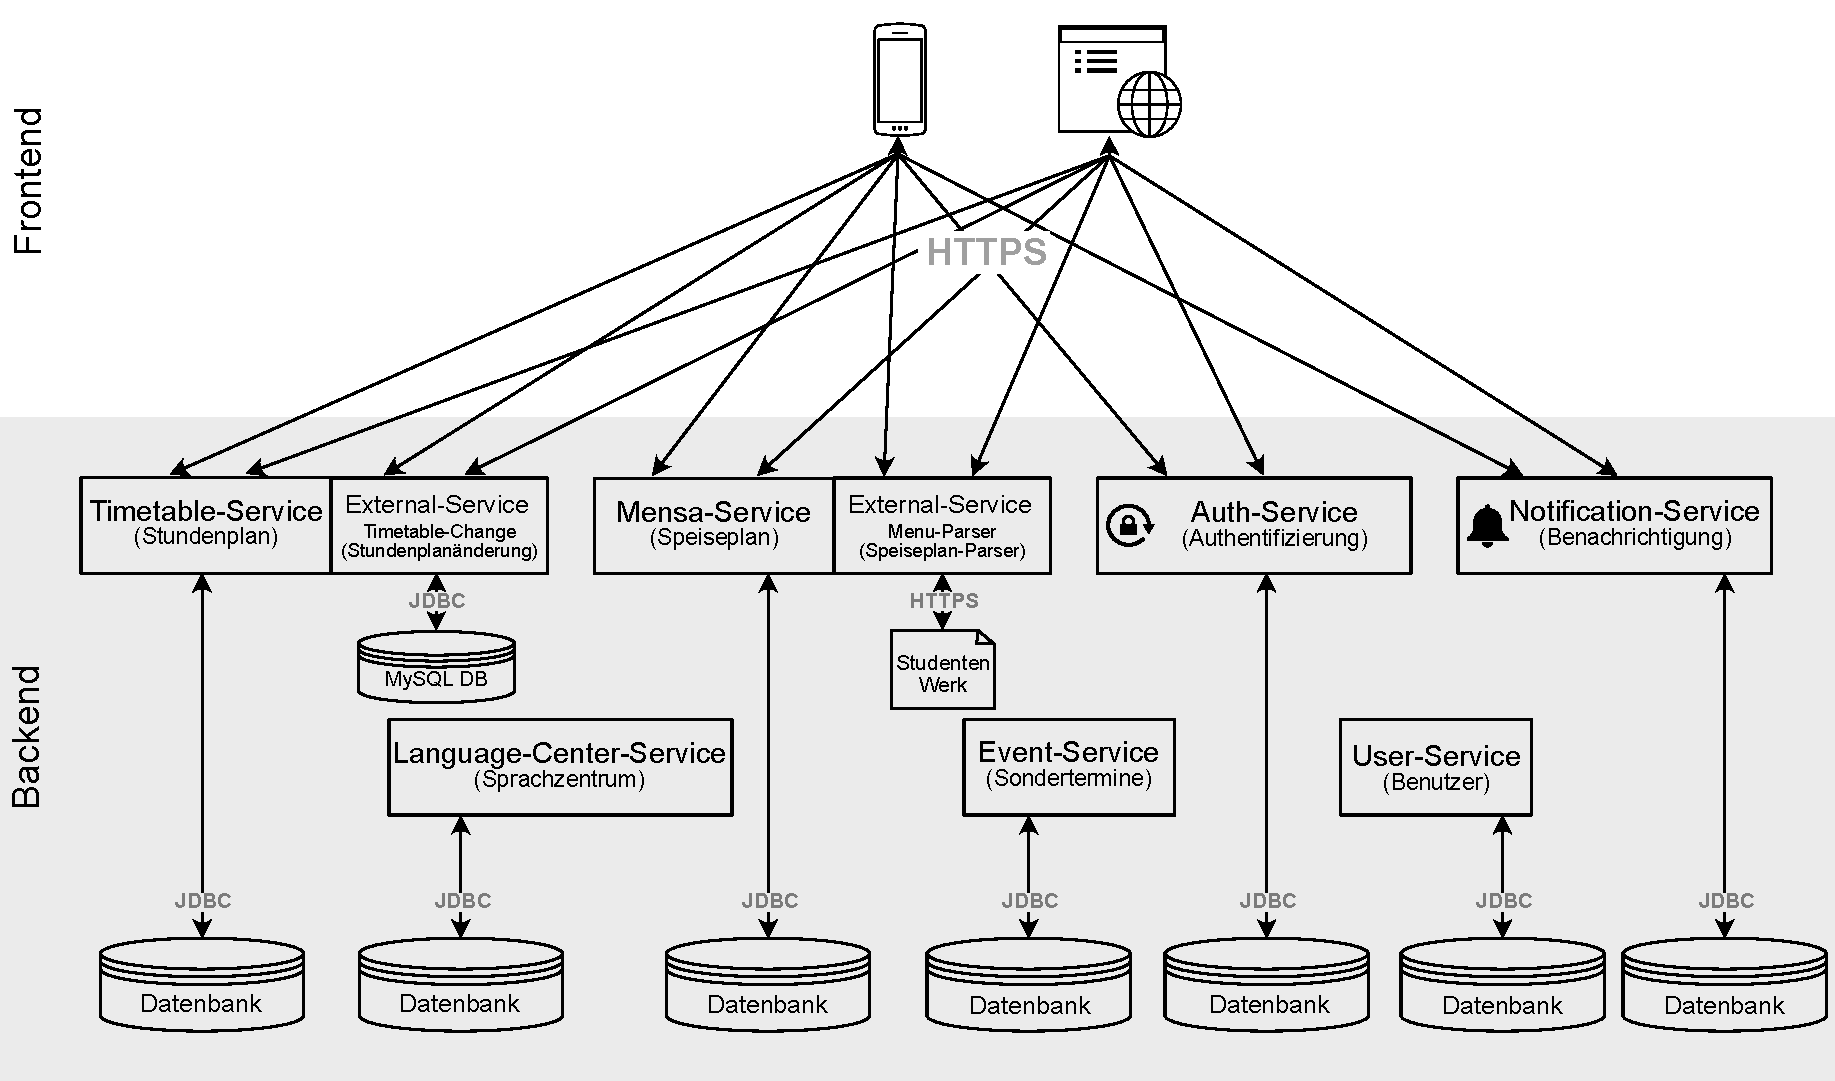
\includegraphics[width=\pictureWidth cm + 2cm]{Bilder/Kapitel_3/app_architektur_no_proxy.pdf}
\caption{Hochschull-APP Architektur ohne Gateway\label{fig:architekturnoproxy}}
\end{figure}

Eine weitere Funktion des Gateways ist die Versionsverwaltung der Services, da dieses Projekt lediglich den Prototypen implementiert und in Zukunft noch weitere Releases erscheinen werden. Deshalb und wegen der bereits genannten Vorteile wird im Prototyp ein \ac{API}-Gateway eingebunden.

\begin{figure}[H]
\centering
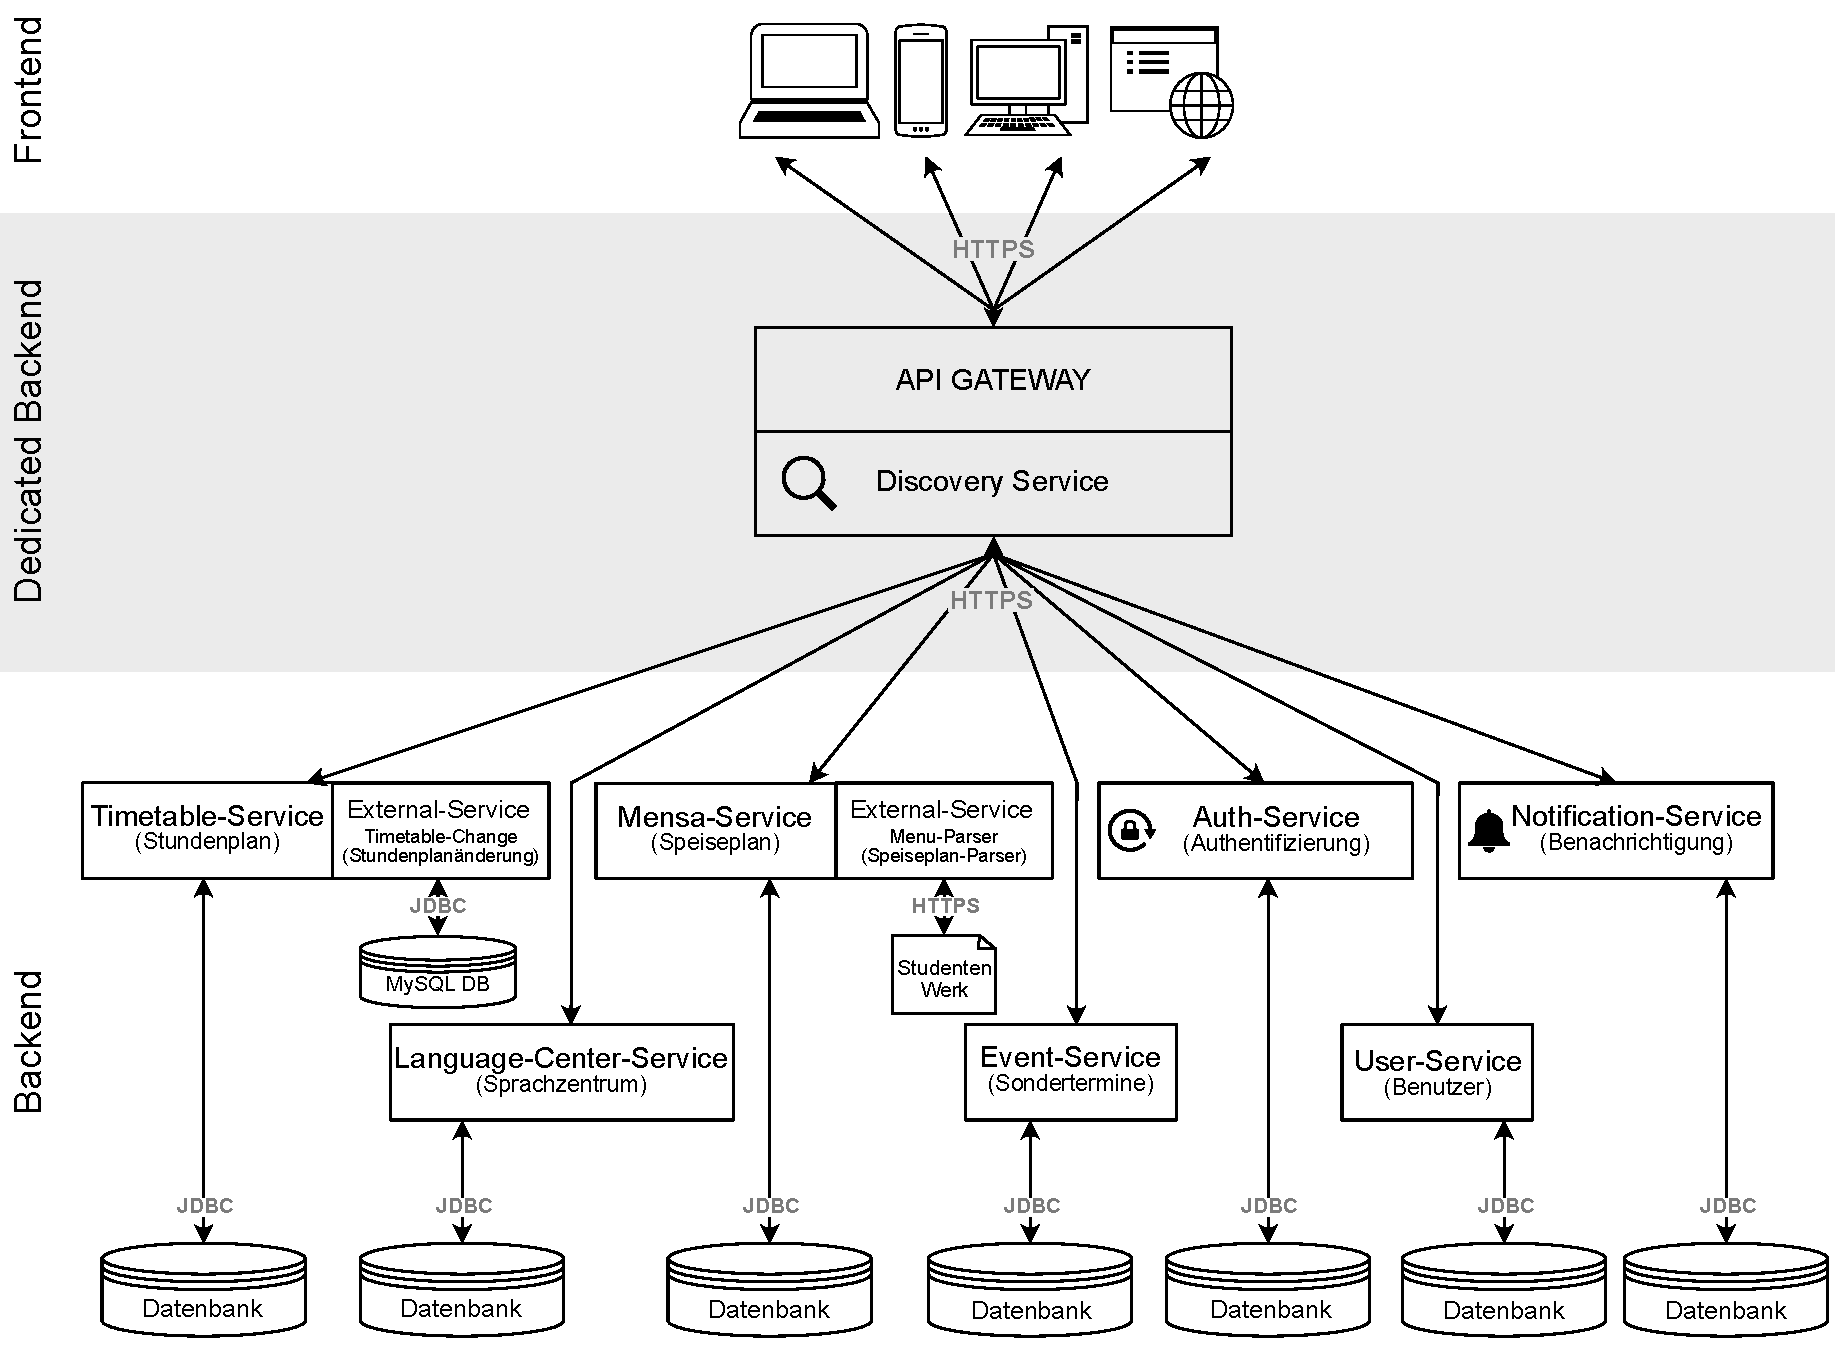
\includegraphics[width=\pictureWidth cm + 2cm]{Bilder/Kapitel_3/app_architektur_proxy.pdf}
\caption{Hochschul-APP Architektur mit Gateway\label{fig:architekturwithproxy}}
\end{figure}

Für die Implementierung des Gateways bieten sich ähnlich wie beim Microservice Framework zahlreiche Alternativen. Darunter sind unter anderen \textit{NGINX}, \textit{Spring Cloud Gateway}, \textit{Zuul} und \textit{KrakenD}. Da die Wahl des Microservice Frameworks jedoch bereits auf \textit{Spring Boot} gefallen ist, wurde die Auswahl der \ac{API}-Gateway Frameworks auf lediglich zwei Kandidaten reduziert, welche bereits in Verbindung mit \textit{Spring} getestet wurden und mit dem Framework harmonieren. Diese Frameworks sind \textit{Zuul} und \textit{Spring Cloud Gateway}.\\
\linebreak
Auch zwischen diesen beiden Frameworks bedarf es jedoch kaum eines aufwändigen Vergleichs, da die von \textit{Spring} entwickelte Gateway Implementierung auf der Basis von \textit{Zuul} implementiert wurde und dieses in Zukunft auch endgültig in Verbindung mit \textit{Spring Boot} ablösen soll. Zudem wurde der Support für \textit{Zuul} in der Version 1.0 eingestellt, was potentielle Sicherheitslücken nicht ausschließen lässt. Neuere Versionen des Frameworks werden von \textit{Spring} ohnehin nicht mehr unterstützt.

\section{Service Registrierung und Discovery}
\label{sec:registryanddiscovery}

Durch die Nutzung des \ac{API}-Gateways wurde die Auslagerung der Funktionalitäten in dezentrale Einheiten ermöglicht. Das bringt, wie bereits erwähnt, einige Vorteile mit sich, erfordert jedoch auch, dass das Gateway selbst die Adressen der einzelnen Services kennt. Diese müssen sich dadurch mit ihren physischen Adressen beim Gateway oder einer anderen zentralen Instanz registrieren. Hierfür wurde beim Prototypen der Hochschul-\ac{App} ein Discovery Server eingebaut. Dieser kümmert sich um das Load-Balancing, verteilt die Anfragen zwischen den Instanzen und leitet die Anfragen an eine ausgefallene Instanz an den passenden Backup Service weiter.\\
\linebreak
Für die konkrete Entwicklung dieser Discovery Funktion gibt es eine Reihe bewährter open-source Lösungen. Zu diesen gehören Frameworks, die auf die Konsistenz der Services ausgelegt sind, wie \textit{Apache Zookeeper}, \textit{Doozer} und \textit{Etcd}, jedoch auch Frameworks, die auf dedizierte Lösungen setzen, um sich auf Load-Balancing und die eigentliche Service Discovery zu konzentrieren, wie \textit{netflix Eureka}, \textit{Spotify DNS}, \textit{SkyDNS}, \textit{NSQ} oder \textit{SmartStack}\autocite[][]{cloud_discovery}.
% referenziert http://jasonwilder.com/blog/2014/02/04/service-discovery-in-the-cloud/
\\
\linebreak
Alle Frameworks bringen bestimmte Vor- und Nachteile mit sich, wobei für die eigentliche Implementierung der Hochschul-\ac{App} prinzipiell jedes der genannten Framework verwendet werden kann. Deshalb wird bei der Wahl des Discovery Frameworks das Hauptaugenmerk auf die Einbindung in das \textit{Spring} Framework gelegt. Speziell n der \textit{Spring Cloud} existieren bereits Lösungen für dieses Konzept, von denen eines das oben genannte \textit{Netflix Eureka} ist. Dieses baut auf Services aus dem \textit{Netflix \ac{OSS}} auf, aus dem auch einige Konzeote in \textit{Spring Cloud} genutzt werden, weshalb sich \textit{Netflix Eureka} perfekt für die Nutzung im Prototypen der neuen Hochschul-\ac{App} eignet.

\section{Benachrichtigung}
\label{sec:notification}

Da es technisch nicht möglich ist, über eine reine Datenschnittstelle Benachrichtigungen an die aufrufenden Clients zu senden, weil nie klar ist, welche Clients den Dienst nutzen, muss ein Benachrichtigungsservice genutzt werden, bei dem sich die Clients registrieren können, um über mögliche Änderungen informiert zu werden. Hierbei bieten sich in der Praxis zwei Alternativen, eine  Push-Benachrichtigungs-\ac{API} selbst entwickeln oder das Nutzen von Drittanbieter Software mit Cloud-Lös\-ungen. Da das Implementierung und Testen solcher Anwendungen sehr aufwändig ist, fällt die eigene Entwicklung dabei aus den möglichen Umsetzungen heraus\autocite[][]{webpush}.
%ref https://golb.hplar.ch/2019/08/webpush-java.html
\\
\linebreak
Deswegen wird auf eine Drittanbieter Lösung bei der Prototyp Entwicklung zurückgegriffen. Diese kümmern sich selbstständig um die Unterstützung unterschiedlicher Anwendungen und der Verschlüsselung der Benachrichtigungen. Eine weit verbreitete und mittlerweile gut getestete Lösung ist das von Google entwickelte \ac{FCM}. \ac{FCM} ermöglicht plattformübergreifende Benachrichtigungen mit der zusätzlichen Unterstützung von mobilen Endgeräten, was im Fokus der Entwicklung der neuen Hochschul-\ac{App} liegt\autocite[][]{firebase_home}. Die kostenlose Lizenz für \ac{FCM} ist für die Hochschull-\ac{App} mehr als ausreichend. Es können täglich bis zu 20.000 Benachrichtigungen mit einem Nachrichteninhalt von 4\ac{kB} an Clients versendet werden. Das entspricht um die 4096 Buchstaben pro Nachricht. Ein weiteres Argument für die Verwendung von \ac{FCM} ist die einfache Einbindung des \textit{Firebase Admin \ac{SDK}} über Maven. Dieses erlaubt die Konfiguration der Authentifizierung, Registrierung und des Versenden von Nachrichten über einen Service und über die Programmiersprache Java.
